\documentclass[final,3p,times,twocolumn]{elsarticle}

\makeatletter
\def\ps@pprintTitle{%
   \let\@oddhead\@empty
   \let\@evenhead\@empty
   \let\@oddfoot\@empty
   \let\@evenfoot\@oddfoot
}
\makeatother

\usepackage{graphicx}
\usepackage{amssymb}

\begin{document}

\begin{frontmatter}

\title{An Implementation of Preferential Deletion in Dynamic Models of Web-Like Networks}
\author{Carlos Santiago Bañón}
\address{College of Engineering and Computer Science - University of Central Florida - Orlando, FL}

\begin{abstract}
This paper attempts to replicate the preferential deletion model for generating random graphs defined by Narsingh Deo and Aurel Cami. In this study, the data brought forth by this new implementation agrees seamlessly with the original model. The data presented by Deo and Cami is validated and corroborated, as similar results are found. Further, this paper serves to once again show that the expected fraction of nodes with degree $k$ in the graph generated by this process does indeed decrease asymptotically as $k^{-1 - (\frac{2p}{2p - 1})}$.
\end{abstract}

\begin{keyword}
Web-Like Networks \sep Interconnection Networks \sep Dynamic Random Graph Modeling \sep Preferential Node Deletion \sep Scale-Free \sep Power-Law Degree Distribution
\end{keyword}

\end{frontmatter}

\section{Introduction}
\label{S:1}

The purpose of this paper is to replicate the results and conclusions obtained by Narsingh Deo and Aurel Cami in their 2005 paper \textit{Preferential Deletion in Dynamic Models of Web-Like Networks}. In their paper, they carefully study the properties of “\textit{web-like}” networks, which they define as “real-life networks such as the network of phone calls, power-distribution networks, citation network, science-collaboration network, movie-actor collaboration network, the network of sexual contacts, neural networks, and various infrastructure networks.” $^{[1]}$

They begin their paper by introducing this concept, following with a discussion on how to properly simulate such networks. Quickly stating that the Erdös-Rényi model does not provide an accurate picture for these networks, they propose a new model: the \textit{Preferential Deletion Model}.

This model focuses on mirroring the properties of a dynamic random graph model, which they formally define as “a discrete-time process which starts out with a small fixed graph and in each subsequent time step a new node is added to the graph or an existing node is deleted from the graph.” $^{[1]}$ For their model, this process of adding and deleting nodes is controlled by some stochastic rules, which are described in the formal definition of the model below.

\section{Notation}
\label{S:2}

As this paper is an implementation of the paper by Deo and Cami, the same notation is used, specified in Figure 1.

\section{Definition of the Preferential Deletion Model}
\label{S:3}

Let $G_1$ be a graph that begins with a single node and a self-loop. For each discrete time step $t + 1$, $t > 0$, either one of these processes can occur:

\subsection{Birth Process}

Deo and Cami define the birth process as follows: “with probability $p$, a new node is added, together with a new edge incident on it. The other end-node $u$ of the new edge is chosen preferentially from among all the existing nodes based on a \textit{linear preferential attachment rule}.” $^{[1]}$

Further, this linear preferential attachment can be defined as:

\begin{equation}
\centering
    \mathbb{P}_{t + 1}[u] = \frac{d_t(u)}{\sum_{w \in V_t} d_t(w)} = \frac{d_t(u)}{2m_t}.
\end{equation}

\begin{figure}[h]
\centering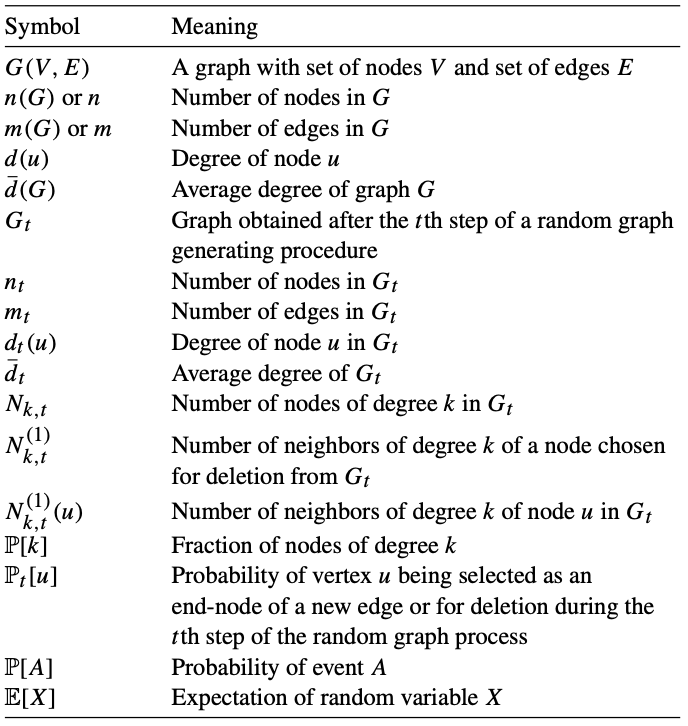
\includegraphics[width=1\linewidth]{notation.png}
\caption{Notation used in this paper.}
\end{figure}

\subsection{Death Process}

If a new node is not created, then a node will be deleted from the list. This process is defined as follows: “with probability $q = 1 - p$, a node $u$ is chosen for deletion along with all the edges incident on it in $G_t$. To make small-degree nodes more likely candidates for deletion than the higher-degree ones, node $u$ is chosen according to the probability distribution defined below.” $^{[1]}$

\begin{equation}
\centering
    \mathbb{P}_{t + 1}[u] = \frac{n_t - d_t(u)}{n^2_t - 2m_t} 
\end{equation}

Finally, they state that, if during any step $t < 0$, the graph becomes empty, then it starts anew with a single node and a self-loop.

\section{Number of Nodes}
\label{S:4}

The original paper begins its discussion regarding the expected number of nodes in the resulting random graph by stating that, based on their model, the graph will seldom vanish. That is, there is a very low probability, shown mathematically as $\mathbb{P}[n_t = 0]$, that the graph will disappear after some step $t > 0$. 
Further, after some derivation, they formally established the expected number of nodes after running their model to be:

\begin{equation}
\centering
    \mathbb{E}[n_t] = (p - q)t + 2q.
\end{equation}

This strongly suggests that the order of growth of $n_t$ is:

\begin{equation}
\centering
    \mathbb{E}[n_t] = \Theta[(p - q)t].
\end{equation}

With this in mind, the new implementation of their model was run with similar parameters in order to test this definition. With the average data collected from the simulations, very similar results were obtained, thereby confirming this mathematical expectation. The expected number of nodes obtained from this new implementation of the model can be seen in Figure 2.

\begin{figure}[h]
\centering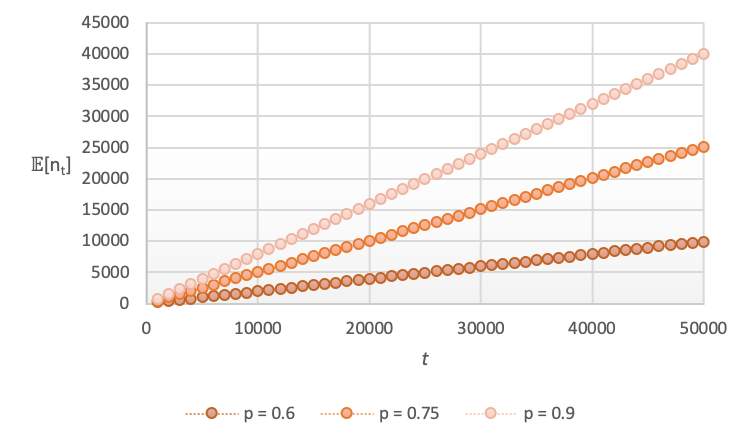
\includegraphics[width=1\linewidth]{nodes.png}
\caption{Expected number of nodes.}
\end{figure}

\section{Number of Edges}
\label{S:5}

Deo and Cami then continue by discussing the expected number of edges in a random graph created by their model. After deriving from various probabilities, the arrive at the conclusion that the expected number of edges of graph $G_t$ can be modeled by the order of:

\begin{equation}
\centering
    \mathbb{E}[m_t] = \Theta[p(p - q)t].
\end{equation}

As before, the new implementation of the model was also used to corroborate these findings. The new results, seen in Figure 3, clearly show an agreement between the original paper and this new implementation. The expected number of edges of graph $G_t$ can be seen in Figure 3.

\begin{figure}[h]
\centering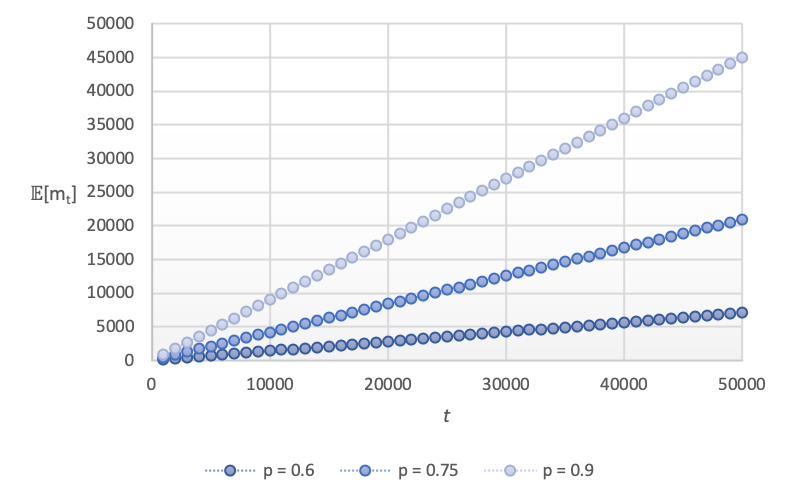
\includegraphics[width=1\linewidth]{edges.png}
\caption{Expected number of edges.}
\end{figure}

\section{Degree Distribution in the First Neighborhood of the Deleted Node}
\label{S:6}

Further, the discussion then shifts to an in-depth analysis of the degree distribution of a random graph $G$ generated with their model. However, Deo and Cami first focus on the degree distribution in the first neighborhood of a deleted node in $G_t$. They formally portray this idea as the expected “number of neighbors of degree $k$ of a node chosen for deletion from $G_t$.” $^{[1]}$ This can be formally defined as:

\begin{equation}
\centering
    \mathbb{E}[N_{k, t}^{(1)}] \approx k\mathbb{E}[N_{k, t}]\mathbb{E}\bigg[\frac{1 - 2\bar{d}_t/n_t}{n_t - \bar{d}_t}\bigg].
\end{equation}

This distribution was also gathered from the new implementation of the model, and this new data can be seen in Figure 4. As evident, the new implementation agrees seamlessly with the original paper.

\begin{figure}[h]
\centering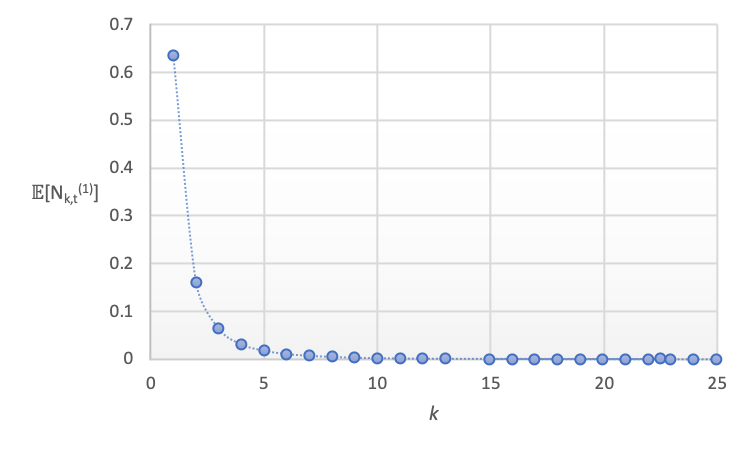
\includegraphics[width=1\linewidth]{degree-distribution.png}
\caption{The expected number of neighbors of degree $k$ of a node chosen for deletion.}
\end{figure}

\section{Degree Distribution}
\label{S:7}

Finally, Deo and Cami turn to the overall degree distribution for a graph $G_t$ generated randomly by their model. Mathematically, they found that “the expected fraction of nodes with degree k in the graph generated by this process decreases asymptotically as $k^{-1 - (\frac{2p}{2p - 1})}$,” and this statistic was also gathered by the new implementation described in this paper.$^{[1]}$ The cumulative degree distribution obtained by the new implementation can be seen in Figure 5. These values match the experimental values produced for the original paper, and thus agree with the mathematical model.

\begin{figure}[h]
\centering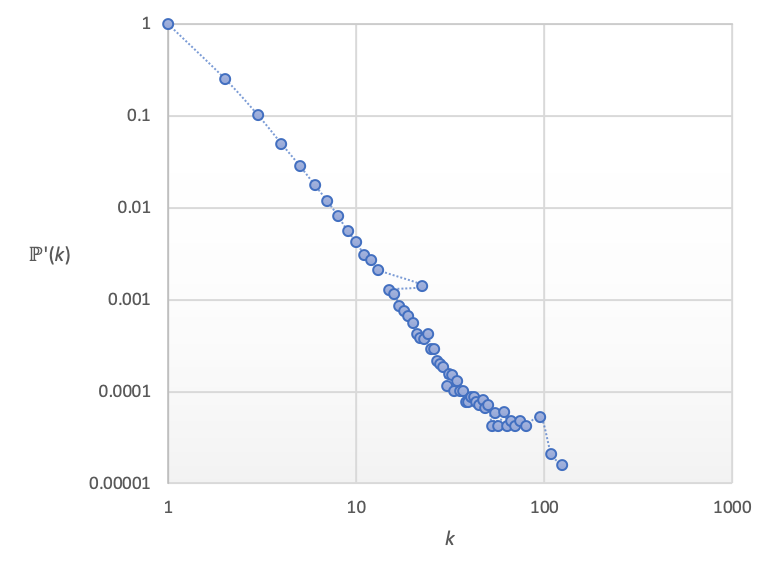
\includegraphics[width=1\linewidth]{cumulative-distribution.png}
\caption{Cumulative degree distribution of the graph generated by the new implementation of the preferential deletion model.}
\end{figure}

\section{Conclusion}
\label{S:8}

With this paper, we can conclude that indeed the results of the original paper can be replicated, and thus gives further validity to the preferential deletion model presented by Deo and Cami. That is, this model generates graphs with asymptotically power-law degree distribution. This then further establishes the model as a very sound way of dynamically generating random graphs for further study of web-like networks. However, this model, as any model, can certainly be improved, and will be the subject of a study in the very near future.

\section{References}
\label{S:9}

$[1]$ N. Deo, A. Cami, Preferential deletion in dynamic models of web-like networks, in: Information Processing Letters, Volume 102, Issue 4, 2007, Pages 156-162.

\end{document}